\documentclass{article}
\usepackage{graphicx} % Required for inserting images
\usepackage{amssymb,amsmath}
\usepackage{caption}
\usepackage{subcaption}
\usepackage{multirow,multicol}
% set spacing in tables

\graphicspath{ {./Img/} }
\title{
CSE 300: Online Assignment\\
}
\author{Md Shamsuzzoha Bayzid, Mahjabin Nahar, Md Shariful Islam Bhuyan,\\ and Md Saidur Rahman}
\date{June 2021}

\begin{document}

\maketitle

\section{Introduction}
This assignment has been designed to assess the preparation of the students in writing scientific articles using \LaTeX. This assignment covers a variety of
components that are commonly used in scientific manuscripts.

\subsection{Equations}

Let $a_{0}$,  $a_{n}$ and  $b_{n}$ are terms of a series. Their definitions are given by \ref{eq1}\\
\vspace{4mm}
\raggedright
\large
\begin{equation} \label{eq1}
$a_{0} = \frac{1}{\pi} \int_{-\pi}^{\pi} f(x) \,dx$\\
\vspace{5mm}
$a_{n} = \frac{1}{\pi} \int_{-\pi}^{\pi} f(x)\cos nx \,dx = 
\frac{1}{\pi} \int_{-\pi}^{\pi} x^2\cos nx \,dx$\\
\vspace{5mm}

$b_{n} = \frac{1}{\pi} \int_{-\pi}^{\pi} f(x)\sin nx \,dx = 
\frac{1}{\pi} \int_{-\pi}^{\pi} x^2\sin nx \,dx$\\
\vspace{2mm} 
\end{equation}

\subsection{Tables}
We wish to place the Table at the bottom of the page.

\subsection{Figures}
We intend to put Figure 1 at the top of a page.



% two images side by side
\begin{figure}
    \centering
    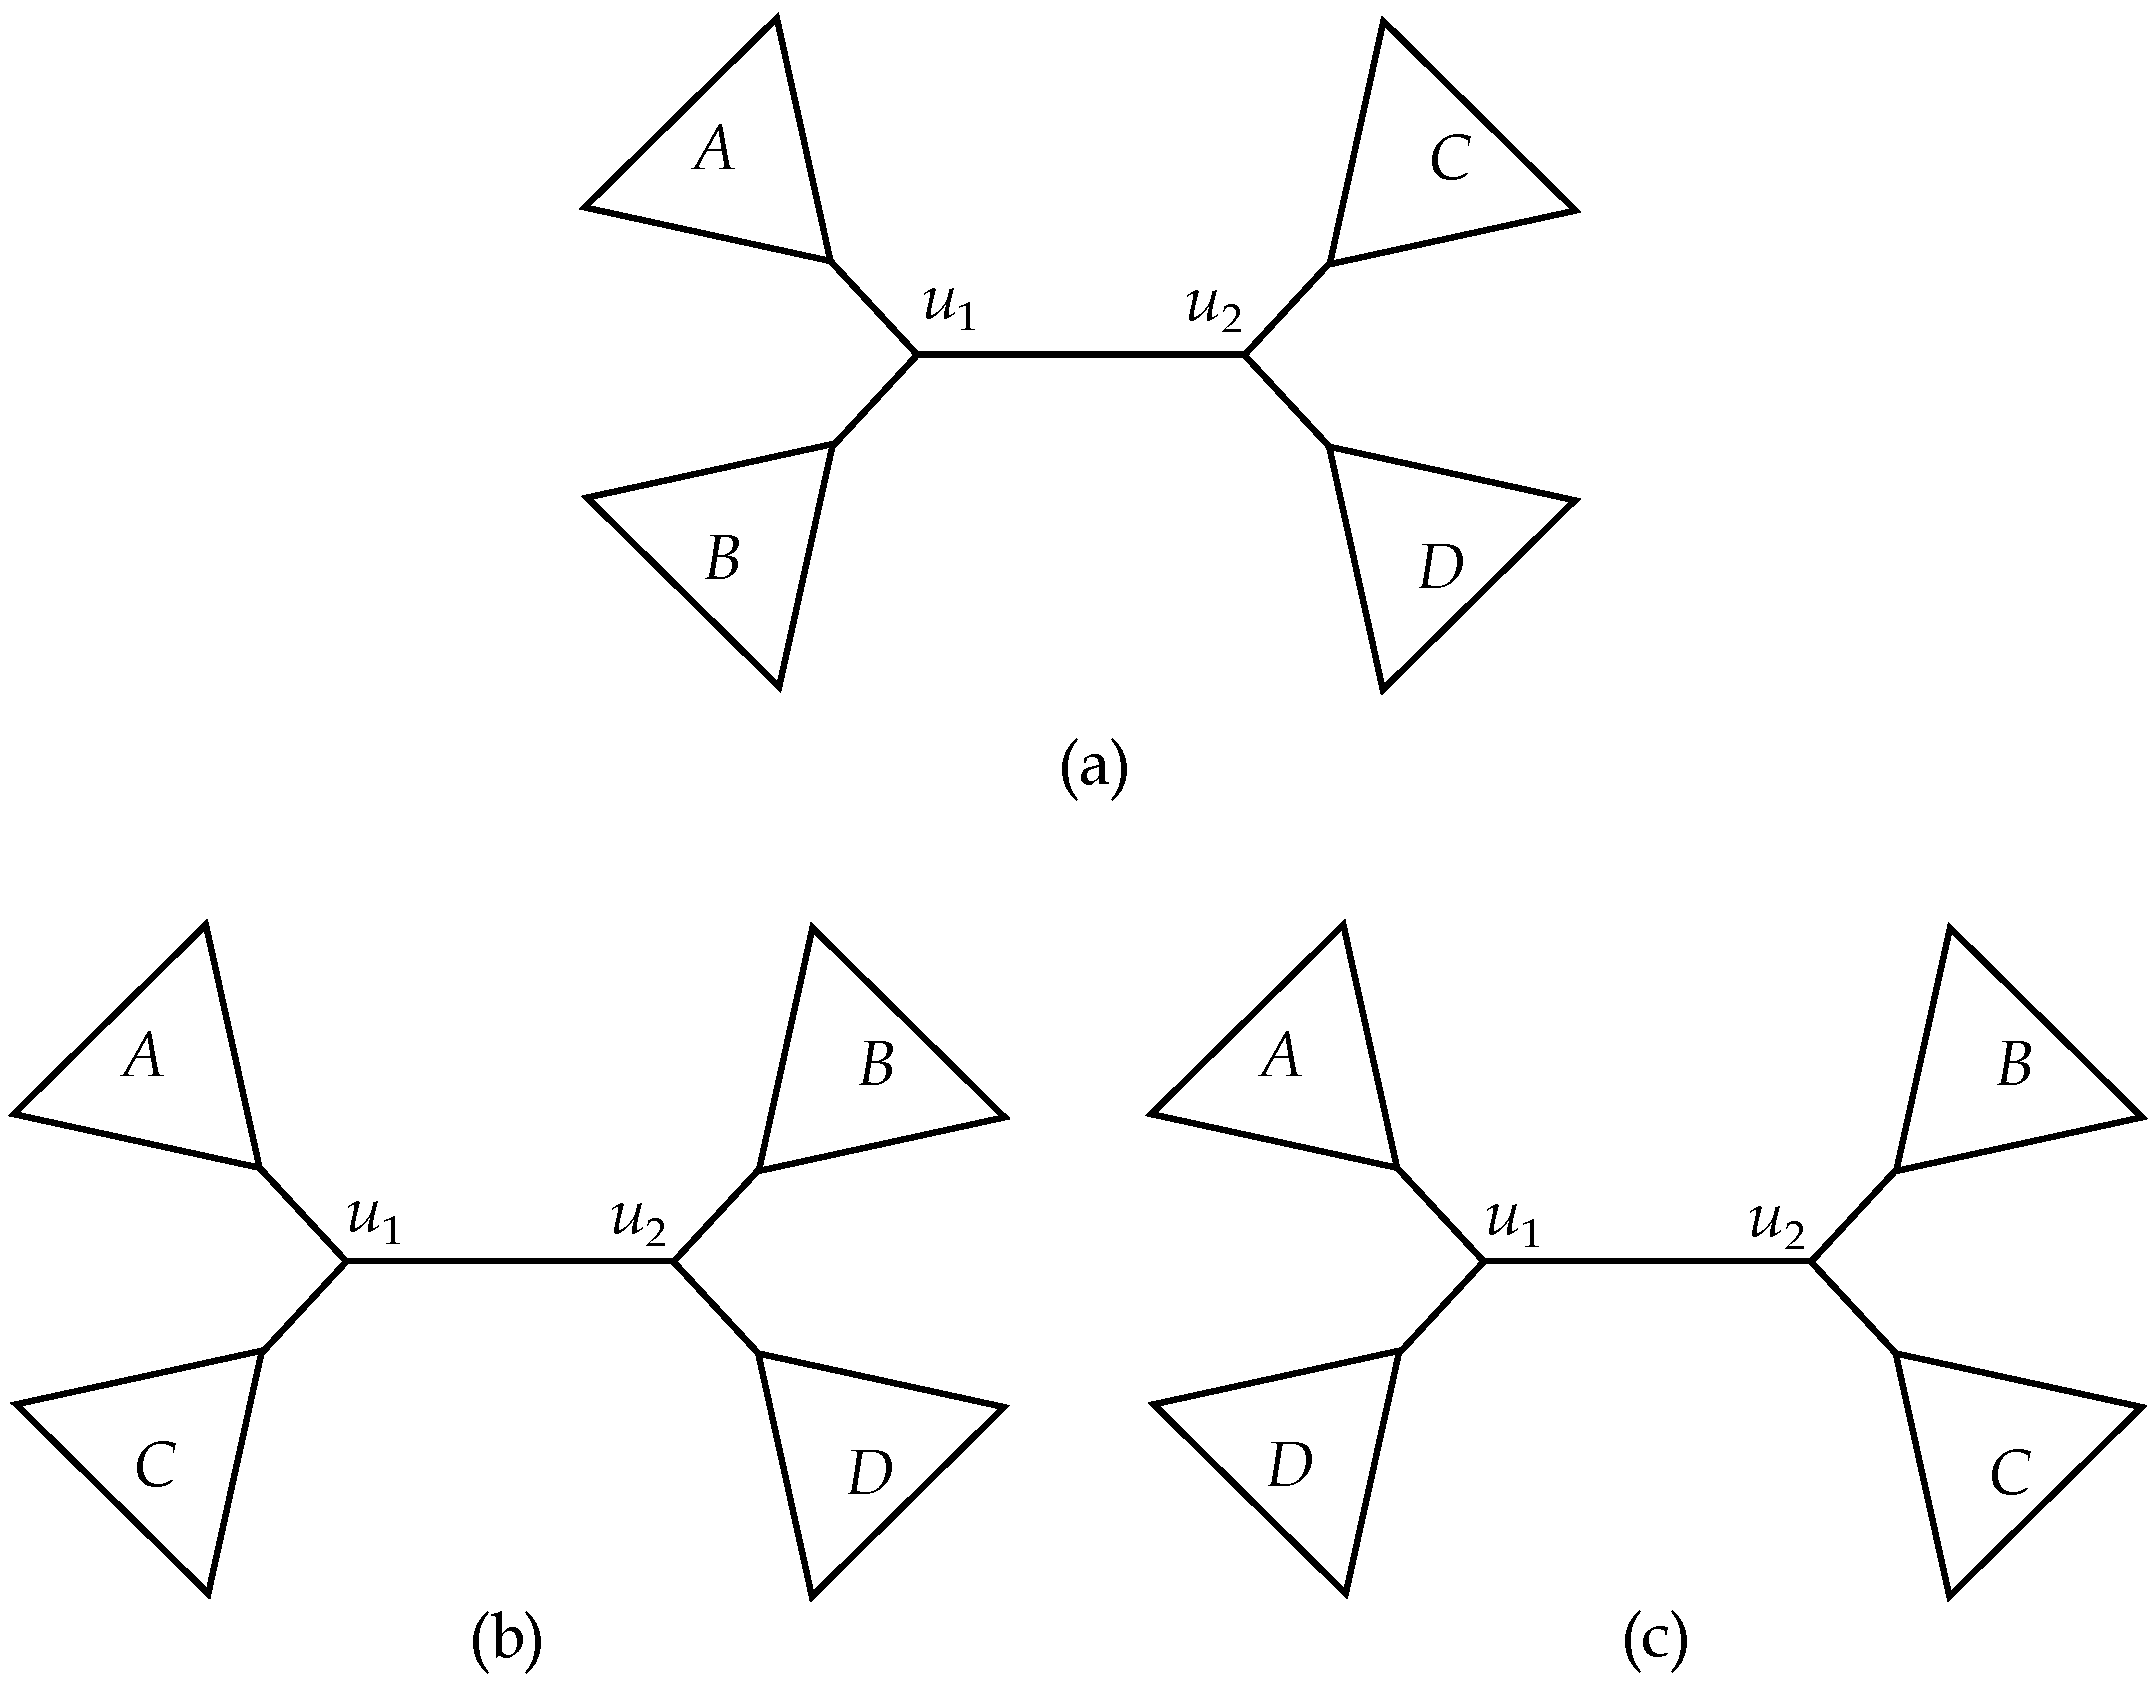
\includegraphics[angle=90,width=0.4\linewidth]{Practice_Problem_4.pdf} 
    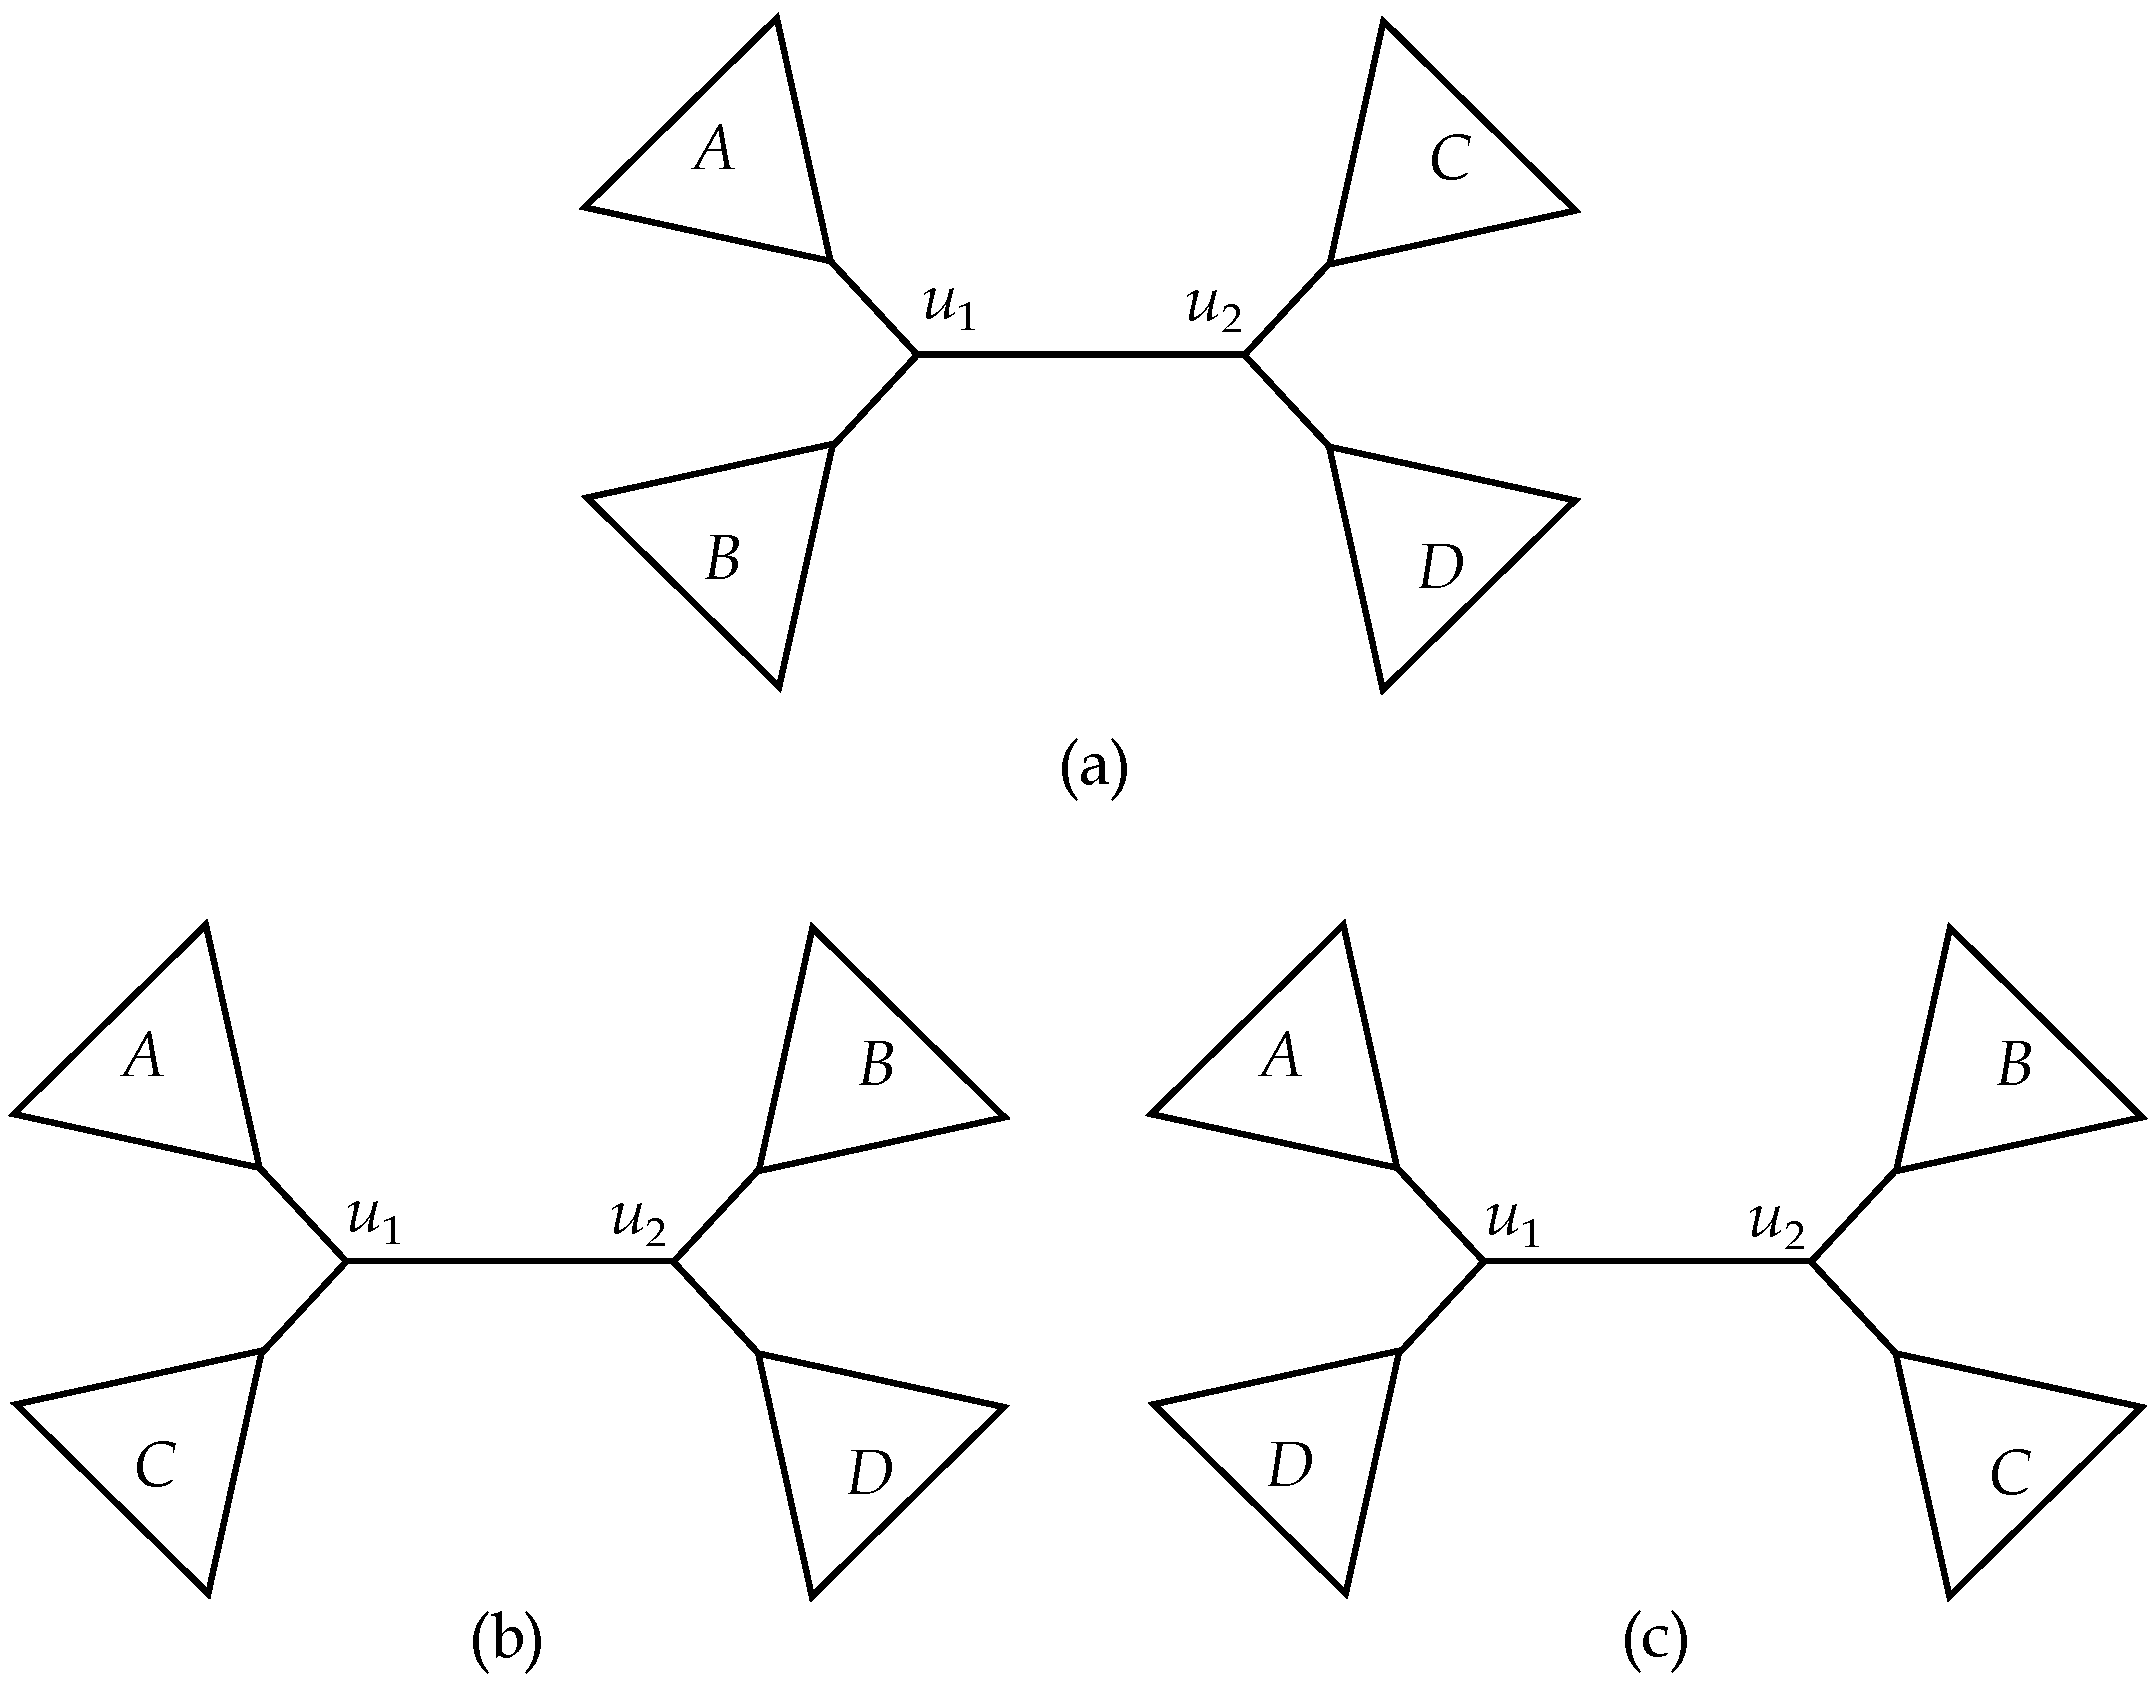
\includegraphics[angle=90,width=0.4\linewidth]{Practice_Problem_4.pdf}
    \caption{\textbf{Side by side same figure}}
    \label{fig:1}
\end{figure}



\newpage
\section{Conclusions}

The major objectives of this assignment are listed below (please do not ignore the font sizes).

\begin{itemize}
    \item \Large To assess the ability of the students in preparing manuscripts in \LaTeX.
    \item \large To assess the ability of the students in preparing manuscripts in \LaTeX.
\end{itemize}

\begin{table}[!h]
    \centering
    \begin{tabular}{|l||l|l|l|}
    \hline
    \multicolumn{4}{|c|}{Item List} \\ \hline
    \multicolumn{1}{|l||}{Item Name or}  &  \multicolumn{1}{|l|}{ALPHA 2 Code} & ALPHA 3 Code& Numeric Code \\
   \multicolumn{1}{|l||}{Product Name} &  &  & \\ \hline
   Item001 & AF & AFG & \begin{tabular}{|c|} 004 \\ \hline \end{tabular} \\ 
   Item002 & AX & ALA & \begin{tabular}{|c|} 008 \\ \hline \end{tabular} \\ 
   Item003 & AL & ALB & \begin{tabular}{|c|} 009 \\ \hline \end{tabular} \\ 
   Item004 & DZ & DZA & \begin{tabular}{|c|c|c|} \hline 012 & 013 & 014\\ \hline \end{tabular} \\ \hline \hline
   Item005 & AS & ASM & \begin{tabular}{|c|} 016 \\ \hline \end{tabular} \\ 
   Item006 & AD & AND & \begin{tabular}{|c|c|} \hline 010 & 020 \\ \hline \end{tabular} \\ 
   Item007 & A) & AGO & \begin{tabular}{|c|c|} \hline 024 & 025 \\ \hline \end{tabular} \\ \hline \hline \hline
    \end{tabular}
\end{table}

\pagebreak

\begin{itemize}
    \item To see if the students can add various basic components (e.g., tables, figures, equations) to a \LaTeX manuscript.
    \item \small To see if the students can leverage the available materials (both offline and online) to do something which has not explicitly been taught in the class.
\end{itemize}




\end{document}
